\documentclass[aspectratio=169]{beamer}
\usepackage{tikz}
\usepackage{graphicx}

\usecolortheme{whale}
\usetikzlibrary{er,positioning}  
\usetikzlibrary{decorations.pathreplacing}
\usetikzlibrary{arrows, decorations.markings}
\usetikzlibrary{shapes.geometric}

\setbeamertemplate{navigation symbols}{}

\definecolor{violet}{rgb}{0.53, 0.0, 0.69}

\definecolor{blue1}{RGB}{126,126,206}
\definecolor{blue2}{RGB}{87,87,192}
\definecolor{blue3}{RGB}{51,51,178}
\definecolor{blue4}{RGB}{27,26,107}

\tikzstyle{every link} = []
\tikzstyle{link} = [>=triangle 60, draw, every link]

\definecolor{attr}{RGB}{10,153,2}

\title{Bases de Datos I}
\subtitle{Teor\'ia del dise\~no: Tercera Forma Normal}
\author[Garc\'ia L., Cardentey V. M.]{
    Lic. V\'ictor M. Cardentey Fundora\\ 
    Dra. Lucina Garc\'ia Hern\'andez
}
\institute[MATCOM-UH]{
    Departamento de Computaci\'on\\
    Facultad de Matem\'atica y Computaci\'on\\
    Universidad de La Habana
}
\date[]{3 de abril de 2023}


\begin{document}
    \maketitle
    \begin{frame}{Si tenemos el conjunto de DFs del universo de atributos}
    \centering
    \LARGE ¿Podemos garantizar la calidad de la base de datos?
    
\end{frame}

{
\setbeamertemplate{background} 
{
    
\includegraphics[width=\paperwidth,height=\paperheight]{img/database-issues.jpg}
}
\begin{frame}
\end{frame}
}

\begin{frame}{Objetivos}
    \begin{enumerate}
        \item Poder extraer las dependencias funcionales existentes en un fen\'omeno a partir de su especificaci\'on y modelaci\'on conceptual.
        \item Poder identificar anomal\'ias en un dise\~no de base de datos relacional.
        \item Poder obtener un dise\~no de base de datos relacional en tercera forma normal.
    \end{enumerate}

    % @TODO ver si mezclamos estos con los del otro fragmento de la conf
\end{frame}


\begin{frame}{La situaci\'on}
    Se desea desarrollar una base de datos para registrar las notas
    de los estudiantes de la carrera en cada una de las asignaturas que
    cursan:
    \begin{itemize}
        \item De cada estudiante se conoce su identificador, su nombre, su grupo y su provincia de residencia.
        \item De cada asignatura se conoce su identificador y su nombre.
        \item Por cada asignatura se conoce la nota que obtuvo el estudiante en la evaluaci\'on final.
    \end{itemize}
    Adem\'as, se conoce que los estudiantes son organizados en los grupos de acuerdo a su provincia.
\end{frame}


\begin{frame}{Primero lo primero}

    \resizebox{\linewidth}{!}{
                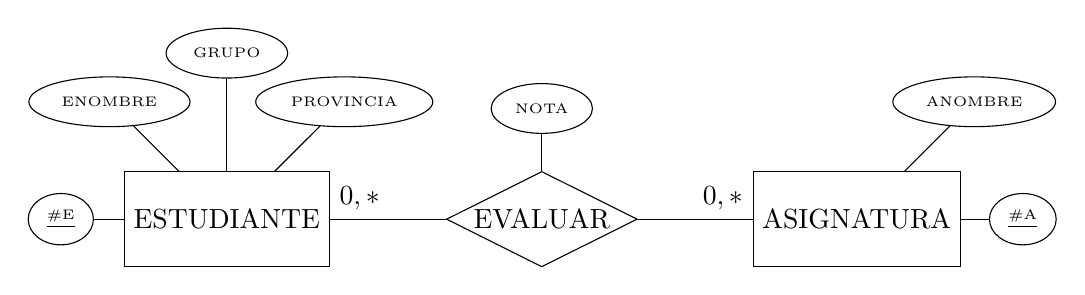
\begin{tikzpicture}[node distance=6em]
                    \tikzstyle{every entity} = [minimum width=2cm, minimum height=1.2cm]
                    \node[entity] (estudiante) {ESTUDIANTE}
                        [sibling distance=3cm]
                        child {node[attribute] [above right of=estudiante] {\tiny PROVINCIA}}
                        child {node[attribute] [above of=estudiante] {\tiny GRUPO}}
                        child {node[attribute] [above left of=estudiante] {\tiny ENOMBRE}}
                        child {node[attribute] [left of=estudiante] {\underline{\tiny \#E}}};
                  
                    \node[entity] (asignatura) at (8,0) {ASIGNATURA}
                    [sibling distance=3cm]
                    child {node[attribute] [right of=asignatura] {\underline{\tiny \#A}}}
                    child {node[attribute] [above right of=asignatura] {\tiny ANOMBRE}};
                    
                  
                    \node[relationship,aspect=2] (evaluar) at (4,0) {EVALUAR}[node distance=4em]
                    child {node[attribute] [above of=evaluar] {\tiny NOTA}};
                    \draw (evaluar.east) -- (asignatura.west) node[above left] {$0,\ast$};
                    \draw (evaluar.west) -- (estudiante.east) node[above right] {$0,\ast$};
                \end{tikzpicture}
            }
\end{frame}


\begin{frame}{Metodolog\'ia para obtener un esquema relacional correcto}
    \begin{enumerate}
        \item Identificar el universo $U$ de atributos del fen\'omeno.
        \item Identificar el conjunto $F$ de las dependencias funcionales que se establecen entre los atributos.
        \item Definir el esquema relacional $R(U,F)$.
    \end{enumerate}
\end{frame}


\begin{frame}{Ejemplo}
    \begin{enumerate}
        \item $U = \{ \textnormal{\#E, ENombre,  Grupo, Provincia, \#A, ANombre, Nota}\}$
    \end{enumerate}

    \onslide<2>{
    \vspace{10mm}

    \centering    
    \large{¿C\'omo podemos obtener $F$ a partir del dise\~no conceptual?}}
\end{frame}

\begin{frame}{Algoritmo de extracci\'on de dependencias funcionales}
    \begin{enumerate}
        \item<2-> Por cada conjunto de entidades con un conjunto de atributos $X \subseteq U$,
        se a\~nade la dependencia funcional $K \to X$ donde $K$ es la llave del conjunto de entidades.
        \item<3-> Por cada conjunto de interrelaciones se toma su llave $K$ y se a\~nade la
        dependencia funcional $K \to K$. Adem\'as, por cada conjunto de entidades en un extremo
        de cardinalidad m\'axima 1 en la interrelaci\'on, se a\~nade la dependencia funcional $K - K_E \to K_E$ donde
        $K_E$ es la llave del conjunto de entidades.
        \item<4-> Por cada agregaci\'on con un conjunto de atributos $X \subseteq U$ se a\~nade la dependencia
        funcional $K \to X$ donde $K$ es la llave del conjunto de interrelaciones que encierra la agregaci\'on.
        \item<5-> A\~nadir aquellas dependencias funcionales asociadas a otras restricciones del negocio
        especificadas en los requerimientos.
    \end{enumerate}
        
\end{frame}


\begin{frame}{Ejecutando el algoritmo}
    \centering
    \resizebox{!}{2.5cm}{
        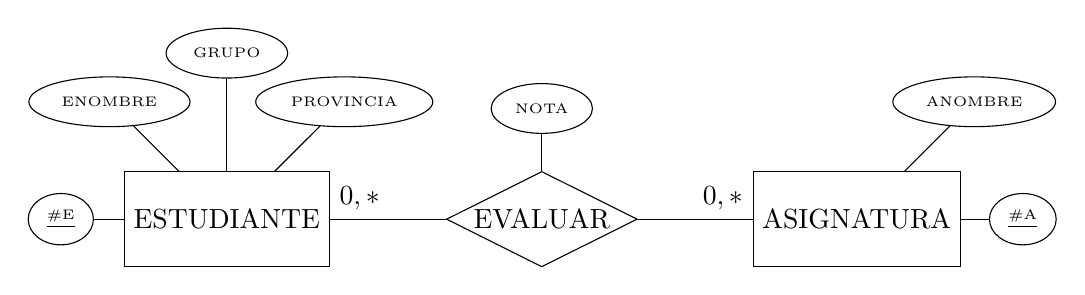
\begin{tikzpicture}[node distance=6em]
            \tikzstyle{every entity} = [minimum width=2cm, minimum height=1.2cm]
            \node[entity] (estudiante) {ESTUDIANTE}
                [sibling distance=3cm]
                child {node[attribute] [above right of=estudiante] {\tiny PROVINCIA}}
                child {node[attribute] [above of=estudiante] {\tiny GRUPO}}
                child {node[attribute] [above left of=estudiante] {\tiny ENOMBRE}}
                child {node[attribute] [left of=estudiante] {\underline{\tiny \#E}}};
            
            \node[entity] (asignatura) at (8,0) {ASIGNATURA}
            [sibling distance=3cm]
            child {node[attribute] [right of=asignatura] {\underline{\tiny \#A}}}
            child {node[attribute] [above right of=asignatura] {\tiny ANOMBRE}};
            
            
            \node[relationship,aspect=2] (evaluar) at (4,0) {EVALUAR}[node distance=4em]
            child {node[attribute] [above of=evaluar] {\tiny NOTA}};
            \draw (evaluar.east) -- (asignatura.west) node[above left] {$0,\ast$};
            \draw (evaluar.west) -- (estudiante.east) node[above right] {$0,\ast$};
        \end{tikzpicture}
    }
        \vspace{3mm}


        \begin{enumerate}
            \item<2-> Se tienen los conjuntos de entidades ESTUDIANTE y ASIGNATURA:\begin{itemize}
                \item $\textnormal{\#E} \to \textnormal{ENombre, Grupo, Provincia}$
                \item $\textnormal{\#A} \to \textnormal{ANombre}$
            \end{itemize}
            \item<3-> Se tiene el conjunto de interrelaciones EVALUAR: \begin{itemize}
                \item $\textnormal{\#E,\#A} \to \textnormal{\#E,\#A}$
            \end{itemize}
            \item<4-> Se tiene la agregaci\'on ASIGNATURA-EVALUADA \begin{itemize}
                \item $\textnormal{\#E, \#A} \to \textnormal{Nota}$
            \end{itemize}
            \item<5-> A\~nadimos las restricciones planteadas en la especificaci\'on: \begin{itemize}
                \item $\textnormal{Provincia} \to \textnormal{Grupo}$
            \end{itemize}
        \end{enumerate}
\end{frame}

\begin{frame}{Continuemos con el ejemplo}
    \begin{enumerate}
        \item $U = \{ \textnormal{\#E, ENombre,  Grupo, Provincia, \#A, ANombre, Nota}\}$
        \item $F = \{$ \\
        \hspace{10mm} $\textnormal{\#E} \to \textnormal{ENombre, Grupo, Provincia}$\\
        \hspace{10mm} $\textnormal{\#A} \to \textnormal{ANombre}$\\
        \hspace{10mm} $\textnormal{\#E,\#A} \to \textnormal{\#E,\#A}$\\
        \hspace{10mm} $\textnormal{\#E, \#A} \to \textnormal{Nota}$\\
        \hspace{10mm} $\textnormal{Provincia} \to \textnormal{Grupo}$\\
        $\}$
        \item Definimos el esquema relacional $\textbf{Evaluaciones}(U,F)$ con llave \#E, \#A 
    \end{enumerate}

    \note{@NOTE aki' se pone una trivial expli'citamente (spoiler). Provincia->Grupo es una externa al merx}
\end{frame}

\begin{frame}{¿Es este un buen dise\~no? \only<2>{(Redundacia)}\only<3>{(Anomal\'ia de inserci\'on)}}
    \centering
    \begin{tabular}{ccccccc}
        \underline{\#E} & ENombre & Grupo & Provincia & \underline{\#A} & ANombre & Nota\\
        $e_1$ & Juan & {\color<2>{orange}111} & {\color<2>{orange} La Habana} & $a_1$ & An\'alisis & 3\\
        $e_1$ & Juan & {\color<2>{orange}111} & {\color<2>{orange} La Habana} & $a_2$ & L\'ogica & 2\\
        $e_1$ & Juan & {\color<2>{orange}111} & {\color<2>{orange} La Habana} & $a_3$ & \'Algebra & 4\\
        $e_1$ & Juan & {\color<2>{orange}111} & {\color<2>{orange} La Habana} & $a_4$ & Programaci\'on & 5\\
        $e_3$ & Pedro & {\color<2>{orange}111} & {\color<2>{orange} La Habana} & $a_3$ & \'Algebra & 4\\
        $e_2$ & Mar\'ia & {\color<2>{blue}112} & {\color<2>{blue} Matanzas} & $a_1$ & An\'alisis & 3\\
        $e_2$ & Mar\'ia &  {\color<2>{blue}112} & {\color<2>{blue} Matanzas} & $a_2$ & L\'ogica & 3\\
        $e_4$ & Rita &  {\color<2>{blue}112} & {\color<2>{blue} Mayabeque} & $a_2$ & L\'ogica & 3\\
        $e_4$ & Rita &  {\color<2>{blue}112} & {\color<2>{blue} Mayabeque} & $a_4$ & Programaci\'on & 4\\
        $e_5$ & Carlos &  {\color<2>{green}113} & {\color<2>{green} Pinar del R\'io} & $a_3$ & \'Algebra & 3
    \end{tabular}
    \vspace{5mm}

    \centering
    \only<2>{{\textcolor{red}{¿Es necesaria esta redundancia?}}}
    \only<3-4>{
        {¿Se pudiera insertar un alumno que todav\'ia no ha recibido evaluaciones?}\\[2mm]
        \begin{tabular}{ccccccc}
            {\color<4>{red}$e_6$} & Marcos & 111 & La Habana & {\color<4>{red}NULL} & NULL & NULL
            
        \end{tabular}
        }

    % @TODO la de insercio'n ponla antes de la redundancia, ya q esta u'ltima es una consecuencia. Pon la redundancia de u'ltima
\end{frame}

\begin{frame}{¿Es este un buen dise\~no? (Anomal\'ia de eliminaci\'on)}
    \centering
    \begin{tabular}{ccccccc}
        \underline{\#E} & ENombre & Grupo & Provincia & \underline{\#A} & ANombre & Nota\\
        $e_1$ & Juan & 111 & La Habana & $a_1$ & An\'alisis & 3\\
        $e_1$ & Juan & 111 & La Habana & $a_2$ & L\'ogica & 2\\
        $e_1$ & Juan & 111 & La Habana  & $a_3$ & \'Algebra & 4\\
        $e_1$ & Juan & 111 & La Habana & $a_4$ & Programaci\'on & 5\\
        $e_3$ & Pedro & 111 & La Habana & $a_3$ & \'Algebra & 4\\
        $e_2$ & Mar\'ia & 112 &  Matanzas & $a_1$ & An\'alisis & 3\\
        $e_2$ & Mar\'ia &  112 & Matanzas & $a_2$ & L\'ogica & 3\\
        $e_4$ & Rita & 112 & Mayabeque & $a_2$ & L\'ogica & 3\\
        $e_4$ & Rita &  112 & Mayabeque & $a_4$ & Programaci\'on & 4\\
        \onslide<-1>{
        $e_5$ & Carlos &  113 & Pinar del R\'io & $a_3$ & \'Algebra & 3
        }
    \end{tabular}
    \vspace{5mm}

    \only<1>{
        ¿Qu\'e ocurre si se eliminan las notas del estudiante $e_5$?
    }
    \only<2>{
        \textcolor{red}{Se pierde la informaci\'on relacionada con la provincia Pinar del R\'io y el grupo C113}
    }

\end{frame}


\begin{frame}{¿Es este un buen dise\~no? (Anomal\'ia de modificaci\'on)}
    \centering
    \begin{tabular}{ccccccc}
        \underline{\#E} & ENombre & Grupo & Provincia & \underline{\#A} & ANombre & Nota\\
        $e_1$ & Juan & 111 & {\color<2>{red} La Habana} & $a_1$ & An\'alisis & 3\\
        $e_1$ & Juan & 111 & {\color<2>{red} La Habana} & $a_2$ & L\'ogica & 2\\
        $e_1$ & Juan & 111 & {\color<2>{red} La Habana} & $a_3$ & \'Algebra & 4\\
        $e_1$ & Juan & 111 & {\color<2>{red} La Habana} & $a_4$ & Programaci\'on & 5\\
        $e_3$ & Pedro & 111& La Habana & $a_3$ & \'Algebra & 4\\
        $e_2$ & Mar\'ia & 112 & Matanzas & $a_1$ & An\'alisis & 3\\
        $e_2$ & Mar\'ia &  112 &  Matanzas & $a_2$ & L\'ogica & 3\\
        $e_4$ & Rita &  112 & Mayabeque & $a_2$ & L\'ogica & 3\\
        $e_4$ & Rita &  112 & Mayabeque & $a_4$ & Programaci\'on & 4\\
        $e_5$ & Carlos &  113 & Pinar del R\'io & $a_3$ & \'Algebra & 3
    \end{tabular}
    \vspace{5mm}

    \only<1>{
        ¿Cu\'antas tuplas tendr\'iamos que modificar si queremos cambiar la provincia de Juan?
    }
    \only<2>{
        \textcolor{red}{Todas las tuplas deben ser modificadas en una misma transacci\'on}
    }
  

    % @TODO cambia la pregunta pa no mencionar la palabra "modificar", i.e. "que' tendri'amos q hacer?"
\end{frame}










\begin{frame}{Entonces...}
    \centering
    \Large ¿C\'omo solucionar estas anomal\'ias?
\end{frame}

\begin{frame}{F\'acil...}
    \begin{columns}[T]
        \begin{column}{0.68\linewidth}
            \begin{columns}[T]
                \begin{column}{0.6\textwidth}
                    \begin{center}
                        \textbf{Estudiante}\\[2mm]
        
                        \begin{tabular}{ccc}
                            \underline{\#E} & ENombre & Provincia\\[1mm]
                            \hline
                            $e_1$ & Juan & La Habana\\
                            $e_2$ & Mar\'ia & Matanzas\\
                            $e_3$ & Pedro & La Habana\\
                            $e_4$ & Rita & Mayabeque\\
                            $e_5$ & Carlos & Pinar del R\'io
                        \end{tabular}
                    \end{center}
                \end{column}

                \begin{column}{0.4\textwidth}
                    \begin{center}
                        \textbf{Provincia-Grupo}\\[2mm]
        
                        \begin{tabular}{cc}
                            \underline{Provincia} & Grupo\\[1mm]
                            \hline
                            La Habana & 111\\
                            Matanzas & 112 \\
                            Mayabeque & 112 \\
                            Pinar del R\'io & 113
                            
                        \end{tabular}
                    \end{center}
                \end{column}
                
            \end{columns}

            \begin{center}
                \textbf{Asignatura}\\[2mm]

                \begin{tabular}{cc}
                    \underline{\#A} & ANombre\\[1mm]
                    \hline
                    $a_1$ & An\'alisis\\
                    $a_2$ & L\'ogica \\
                    $a_3$ & \'Algebra\\
                    $a_4$ & Programaci\'on
                    
                \end{tabular}
            \end{center}
            
        \end{column}

        \begin{column}{0.3\linewidth}
            \vspace{6mm}
            \begin{center}
                \textbf{Evaluar}\\[2mm]

                \begin{tabular}{ccc}
                    \underline{\#E} & \underline{\#A} & Nota\\[1mm]
                    \hline
                    $e_1$ & $a_1$ & 3\\
                    $e_1$ & $a_2$ & 2\\
                    $e_1$ & $a_3$ & 4\\
                    $e_1$ & $a_4$ & 5\\
                    $e_3$ & $a_3$ & 4\\
                    $e_2$ & $a_1$ & 3\\
                    $e_2$ & $a_2$ & 3\\
                    $e_4$ & $a_2$ & 3\\
                    $e_4$ & $a_4$ & 4\\
                    $e_5$ & $a_3$ & 3\\
                \end{tabular}
            \end{center}
        \end{column}
    \end{columns}
\end{frame}

\begin{frame}{Formalizando el dise\~no}
    \centering
    \Large{ ¿C\'omo obtener esta soluci\'on?}
\end{frame}

% @TODO hasta aki' la 1ra conf de cd

\begin{frame}{Proyecci\'on de las dependencias funcionales}
    Dados un esquema relacional $R(U,F)$ y un conjunto de atributos
    $Z$ tal que $Z \subseteq U$, la proyecci\'on de un conjunto de dependencias
    funcionales $F$ sobre un conjunto de atributos $Z$ -- denotada
    por $\Pi_Z(F)$ -- consiste en el conjunto de dependencias funcionales
    $X \to Y$ de $F^+$ tales que $XY \subseteq Z$.
    
    $$
        \Pi_Z(F) = \{X \to Y \;|\; F \models X \to Y \land XY \subseteq Z \}
    $$
\end{frame}







\begin{frame}{Descomposici\'on de un esquema relacional}


        %\item $U = \{A_1, A_2,...,A_n\}$  %, $A_i \; (i =1,...,n)$ son atributos
        %simples (Abreviadamente $R = A_1,A_2,...,A_n$)
        La descomposici\'on del esquema relacional $R(U,F)$ se representa por \\[2mm]
        $\rho = \{R_1(U_1,F_1), R_2(U_2,F_2),...,R_n(U_n,F_n)\}$\\[2mm]
        de manera tal que:
        \begin{itemize}
            \item $U = \underset{i = 1}{\overset{n}{\bigcup}} U_i$
            \item Para todo $i = 1,...,n$ se cumple que $F_i = \Pi_{U_i}(F)$ 
        \end{itemize}
\end{frame}


\begin{frame}{Normalizaci\'on de una base de datos relacional}
    \begin{columns}[T]
        \begin{column}{0.48\linewidth}
            \textbf{Estudiante}($U_1$, $F_1$):\\
            $U_1 = \{\textnormal{\#E, ENombre, Provincia}\}$\\
            $F_1 = \{\textnormal{\#E} \to \textnormal{Enombre, Provincia}\}$

        \end{column}

        \begin{column}{0.48\linewidth}
            \textbf{Provincia-Grupo}($U_2$, $F_2$):\\
            $U_2 = \{\textnormal{Provincia, Grupo}\}$\\
            $F_2 = \{\textnormal{Provincia} \to \textnormal{Grupo}\}$
        \end{column}
        
    \end{columns}

    \vspace{10mm}

    \begin{columns}[T]
        \begin{column}{0.48\linewidth}
            \textbf{Asignatura}($U_3$, $F_3$):\\
            $U_3 = \{\textnormal{\#A, ANombre}\}$\\
            $F_3 = \{\textnormal{\#A} \to \textnormal{ANombre}\}$
        \end{column}

        \begin{column}{0.48\linewidth}
            \textbf{Evaluar}($U_4$, $F_4$):\\
            $U_4 = \{\textnormal{\#E, \#A, Nota}\}$\\
            $F_4 = \{\textnormal{\#E, \#A} \to \textnormal{Nota}\}$
        \end{column}
        
    \end{columns}
\end{frame}






\begin{frame}{Formas normales}
    \begin{block}{Primera Forma Normal}
        Un esquema relacional $R(U,F)$ est\'a en primera forma
        normal (1FN) si todos los atributos toman un solo valor del dominio
        subyacente.
        
    \end{block}
\end{frame}

\begin{frame}{La trivial}
    \centering
    \begin{tabular}{ccccccc}
        \underline{\#E} & ENombre & Grupo & Provincia & \underline{\#A} & ANombre & Nota\\
        $e_1$ & Juan & 111 & La Habana & $a_1$ & An\'alisis & 3\\
        $e_1$ & Juan & 111 & La Habana & $a_2$ & L\'ogica & 2\\
        $e_1$ & Juan & 111 & La Habana  & $a_3$ & \'Algebra & 4\\
        $e_1$ & Juan & 111 & La Habana & $a_4$ & Programaci\'on & 5\\
        $e_3$ & Pedro & 111 & La Habana & $a_3$ & \'Algebra & 4\\
        $e_2$ & Mar\'ia & 112 &  Matanzas & $a_1$ & An\'alisis & 3\\
        $e_2$ & Mar\'ia &  112 & Matanzas & $a_2$ & L\'ogica & 3\\
        $e_4$ & Rita & 112 & Mayabeque & $a_2$ & L\'ogica & 3\\
        $e_4$ & Rita &  112 & Mayabeque & $a_4$ & Programaci\'on & 4\\
        $e_5$ & Carlos &  113 & Pinar del R\'io & $a_3$ & \'Algebra & 3
    \end{tabular}
    \vspace{5mm}

    \centering
    \Large \textcolor{red}{Toda relaci\'on se encuentra en primera forma normal}
\end{frame}

\begin{frame}{Dependencia funcional completa}
    Dado un esquema relacional $R(U,F)$ y los atributos $X$, $Y$ de $R$
    (posiblemente compuestos), se dice que $Y$ depende funcional
    y completamente de $X$ si y solo si $Y$ depende funcionalmente de
    $X$ y no depende de alg\'un subconjunto propio de $X$.
\end{frame}

\begin{frame}{¿Qu\'e dependencias funcionales existen en esta relaci\'on?}
    \centering
    \begin{tabular}{ccccccc}
        \underline{\#E} & ENombre & Grupo & Provincia & \underline{\#A} & ANombre & Nota\\
        $e_1$ & Juan & 111 & La Habana & $a_1$ & An\'alisis & 3\\
        $e_1$ & Juan & 111 & La Habana & $a_2$ & L\'ogica & 2\\
        $e_1$ & Juan & 111 & La Habana  & $a_3$ & \'Algebra & 4\\
        $e_1$ & Juan & 111 & La Habana & $a_4$ & Programaci\'on & 5\\
        $e_3$ & Pedro & 111 & La Habana & $a_3$ & \'Algebra & 4\\
        $e_2$ & Mar\'ia & 112 &  Matanzas & $a_1$ & An\'alisis & 3\\
        $e_2$ & Mar\'ia &  112 & Matanzas & $a_2$ & L\'ogica & 3\\
        $e_4$ & Rita & 112 & Mayabeque & $a_2$ & L\'ogica & 3\\
        $e_4$ & Rita &  112 & Mayabeque & $a_4$ & Programaci\'on & 4\\
        $e_5$ & Carlos &  113 & Pinar del R\'io & $a_3$ & \'Algebra & 3
    \end{tabular}
\end{frame}

\begin{frame}{Clasificando dependencias}
    \centering
    \begin{columns}[T]
        \begin{column}{0.2\linewidth}
            
        \end{column}
        \begin{column}{0.3\linewidth}
            {\color<2>{blue}
            \#E, \#A $\to$ ENombre\\
            \#E, \#A $\to$ Grupo\\
            \#E, \#A $\to$ Provincia\\
            \#E, \#A $\to$ ANombre\\
            \vspace{1mm}
            }
            {\color<2>{orange}
            \#E, \#A $\to$ Nota\\
            \#E $\to$ ENombre\\
            \#E $\to$ Grupo\\
            \#E $\to$ Provincia\\
            \#A $\to$ ANombre\\
            Provincia $\to$ Grupo
            }
        \end{column}
        \begin{column}{0.3\linewidth}
            \onslide<2>{
            \vspace{5mm}
            \textcolor{blue}{\Large Incompletas}

            \vspace{20mm}
            \textcolor{orange}{\Large Completas}
            }
        \end{column}
        \begin{column}{0.2\linewidth}
            
        \end{column}
    \end{columns}
        
\end{frame}

\begin{frame}{Formas normales}
    \begin{block}{Segunda Forma Normal}
        Un esquema relacional $R(U,F)$ est\'a en segunda
        forma normal (2FN), si est\'a en 1FN y todos los atributos
        no llaves dependen completamente de la llave.
        
    \end{block}
\end{frame}


\begin{frame}{Llegando hasta segunda}
    \vspace{-5mm}
    \begin{columns}[T]
        \begin{column}{0.68\linewidth}
            \begin{center}
                \textbf{Estudiante}\\[2mm]

                \begin{tabular}{cccc}
                    \underline{\#E} & ENombre & Provincia & Grupo\\[1mm]
                    \hline
                    $e_1$ & Juan & La Habana & {\color<2>{red}111}\\
                    $e_2$ & Mar\'ia & Matanzas & 112\\
                    $e_3$ & Pedro & La Habana & {\color<2>{red}111}\\
                    $e_4$ & Rita & Mayabeque & 112\\
                    $e_5$ & Carlos & Pinar del R\'io & 113\\
                \end{tabular}
            \end{center}
            

               

            \begin{center}
                \textbf{Asignatura}\\[2mm]

                \begin{tabular}{cc}
                    \underline{\#A} & ANombre\\[1mm]
                    \hline
                    $a_1$ & An\'alisis\\
                    $a_2$ & L\'ogica \\
                    $a_3$ & \'Algebra\\
                    $a_4$ & Programaci\'on
                    
                \end{tabular}
            \end{center}
            
        \end{column}

        \begin{column}{0.3\linewidth}
            \vspace{6mm}
            \begin{center}
                \textbf{Evaluar}\\[2mm]

                \begin{tabular}{ccc}
                    \underline{\#E} & \underline{\#A} & Nota\\[1mm]
                    \hline
                    $e_1$ & $a_1$ & 3\\
                    $e_1$ & $a_2$ & 2\\
                    $e_1$ & $a_3$ & 4\\
                    $e_1$ & $a_4$ & 5\\
                    $e_3$ & $a_3$ & 4\\
                    $e_2$ & $a_1$ & 3\\
                    $e_2$ & $a_2$ & 3\\
                    $e_4$ & $a_2$ & 3\\
                    $e_4$ & $a_4$ & 4\\
                    $e_5$ & $a_3$ & 3\\
                \end{tabular}
            \end{center}
        \end{column}
    \end{columns}
\end{frame}

\begin{frame}{Llegando hasta segunda}
    \centering
    \Large \textcolor{red}{Todav\'ia existe redundancia innecesaria}
\end{frame}

\begin{frame}{Dependencia funcional transitiva}
    Dado un esquema relacional $R(U,F)$ y los atributos $X$, $Y$ y $Z$ de
    $R$ (posiblemente compuestos), se dice que $Z$ depende funcional
    y transitivamente de $X$ si y solo si $Y$ y $Z$ dependen funcionalmente
    de $X$ y, adem\'as, $Z$ depende funcionalmente de $Y$.

    Si $Z$ no dependiera funcionalmente de $Y$, entonces se dice que $Y$ y $Z$
    son mutuamente independientes.

    
\end{frame}

\begin{frame}{Dependencia funcional transitiva}

    \begin{columns}[T]
        \begin{column}{0.5\linewidth}
            \begin{center}
                \textbf{Estudiante}\\[2mm]

                \begin{tabular}{cccc}
                    \underline{\#E} & ENombre & Provincia & Grupo\\[1mm]
                    \hline
                    $e_1$ & Juan & La Habana & 111\\
                    $e_2$ & Mar\'ia & Matanzas & 112\\
                    $e_3$ & Pedro & La Habana & 111\\
                    $e_4$ & Rita & Mayabeque & 112\\
                    $e_5$ & Carlos & Pinar del R\'io & 113\\
                \end{tabular}
            \end{center}
            
        \end{column}

        \begin{column}{0.5\linewidth}
            \vspace{15mm}
            \hspace{5mm} \#E $\to$ ENombre\\
            \hspace{5mm} \#E $\to$ Grupo\\
            \hspace{5mm} \#E $\to$ Provincia\\
            \hspace{5mm} Provincia $\to$ Grupo
        \end{column}
        
        
    \end{columns}
    \vspace{5mm}

    \centering
    \onslide<2->{

        \#E $\to$ Provincia,  Provincia $\to$ Grupo $\models$ \#E $\to$ Grupo\\[2mm]
    }
    \onslide<3->{

        \Large \textcolor{red}{Existe una dependencia funcional transitiva}
    }
\end{frame}

\begin{frame}{Formas normales}
    \begin{block}{Tercera Forma Normal}
        Un esquema relacional $R(U,F)$ est\'a en tercera forma normal
        (3FN), si est\'a en 2FN y los atributos no llaves son mutuamente independientes.
        
    \end{block}
\end{frame}


\begin{frame}{Al fin, la tercera}
    \vspace{-3mm}
    \begin{columns}[T]
        \begin{column}{0.68\linewidth}
            \begin{columns}[T]
                \begin{column}{0.6\textwidth}
                    \begin{center}
                        \textbf{Estudiante}\\[2mm]
        
                        \begin{tabular}{ccc}
                            \underline{\#E} & ENombre & Provincia\\[1mm]
                            \hline
                            $e_1$ & Juan & La Habana\\
                            $e_2$ & Mar\'ia & Matanzas\\
                            $e_3$ & Pedro & La Habana\\
                            $e_4$ & Rita & Mayabeque\\
                            $e_5$ & Carlos & Pinar del R\'io
                        \end{tabular}
                    \end{center}
                \end{column}

                \begin{column}{0.4\textwidth}
                    \begin{center}
                        \textbf{Pronvincia-Grupo}\\[2mm]
        
                        \begin{tabular}{cc}
                            \underline{Provincia} & Grupo\\[1mm]
                            \hline
                            La Habana & 111\\
                            Matanzas & 112 \\
                            Mayabeque & 112 \\
                            Pinar del R\'io & 113
                            
                        \end{tabular}
                    \end{center}
                \end{column}
                
            \end{columns}

            \begin{center}
                \textbf{Asignatura}\\[2mm]

                \begin{tabular}{cc}
                    \underline{\#A} & ANombre\\[1mm]
                    \hline
                    $a_1$ & An\'alisis\\
                    $a_2$ & L\'ogica \\
                    $a_3$ & \'Algebra\\
                    $a_4$ & Programaci\'on
                    
                \end{tabular}
            \end{center}
            
        \end{column}

        \begin{column}{0.3\linewidth}
            \vspace{6mm}
            \begin{center}
                \textbf{Evaluar}\\[2mm]

                \begin{tabular}{ccc}
                    \underline{\#E} & \underline{\#A} & Nota\\[1mm]
                    \hline
                    $e_1$ & $a_1$ & 3\\
                    $e_1$ & $a_2$ & 2\\
                    $e_1$ & $a_3$ & 4\\
                    $e_1$ & $a_4$ & 5\\
                    $e_3$ & $a_3$ & 4\\
                    $e_2$ & $a_1$ & 3\\
                    $e_2$ & $a_2$ & 3\\
                    $e_4$ & $a_2$ & 3\\
                    $e_4$ & $a_4$ & 4\\
                    $e_5$ & $a_3$ & 3\\
                \end{tabular}
            \end{center}
        \end{column}
    \end{columns}
\end{frame}


\begin{frame}{Eliminando dependencias problem\'aticas}
    \begin{block}{Cubrimiento minimal}
        Dado dos conjuntos de dependencias funcionales $F$ y $G$, se dice
        que $G$ es un cubrimiento minimal o cobertura irreducible
        de $F$ si se cumple que:
        \begin{enumerate}
            \item $G \equiv F$
            \item $G$ no contiene atributos redundantes
            \item $G$ no contiene dependencias redundantes
        \end{enumerate}
        
    \end{block}
\end{frame}


{
\setbeamertemplate{background} 
{
    
\includegraphics[width=\paperwidth,height=\paperheight]{img/automate.jpg}
}
\begin{frame}
\end{frame}
}


\begin{frame}{Automatizando}
    \begin{block}{Algoritmo para obtener un cubrimiento minimal}
        
        \textbf{Entrada}: Un conjunto de DFs $F$ sobre un universo de atributos $U$.\\
        \textbf{Salida}: Un conjunto de DFs $G$, $G \equiv F$, sin atributos ni dependencias redundantes.
        \textbf{M\'etodo}:
        \begin{enumerate}
            \item A partir de $F$ construir un conjunto de DFs, $F'$, tal que cada DF sea de la forma $X \to A$.
            \item A partir de $F'$ construir un conjunto de DFs, $F''$, donde ning\'un determinante contiene atributos redundates; o sea,
            que para ninguna $X \to A$ en $F'$ y $Z \subset X$ se cumpla que
            $F' - \{X \to A\} \cup \{Z \to A\}$ sea equivalente a $F'$.
            \item A partir de $F''$ construir un conjunto de DFs, $F'''$, que no contenga dependencias
            redundantes; o sea, que para ninguna $X \to A$ en $F''$ el conjunto de
            dependencias funcionales $F'' - \{X \to A\}$ sea equivalente a $F''$.
        \end{enumerate}
    \end{block}
\end{frame}

\begin{frame}{Ejecutando el algoritmo}
    \begin{columns}[T]
        
        \begin{column}{0.25\linewidth}
            
            $AB \to C$\\
            $C \to A$\\
            $BC \to D$\\
            $ACD \to B$\\
            {\color<2-3>{red}$D \to EG$}\\
            $BE \to C$\\
            {\color<2-3>{red}$CG \to BD$}\\
            {\color<2-3>{red}$CE \to AG$}
            
        \end{column}
        \begin{column}{0.25\linewidth}
            
            \onslide<3->{

                $AB \to C$\\
                $C \to A$\\
                $BC \to D$\\
                {\color<5-6>{red}
                $ACD \to B$\\}
                {\color<3>{red}
                $D \to E$\\
                $D \to G$\\
                }
                $BE \to C$\\
                {\color<3>{red}
                $CG \to B$\\
                $CG \to D$\\
                $CE \to A$\\
                $CE \to G$
                }
            }

            
        \end{column}
        \begin{column}{0.25\linewidth}
            \onslide<6->{

            $AB \to C$\\
            $C \to A$\\
            $BC \to D$\\
            {\color<6>{red}
            $CD \to B$\\}
            $D \to E$\\
            $D \to G$\\
            $BE \to C$\\
            {\color<7>{red}
            $CG \to B$\\}
            $CG \to D$\\
            {\color<7>{red}
            $CE \to A$\\}
            $CE \to G$
        }
        \end{column}
        \begin{column}{0.25\linewidth}
            \onslide<8->{

            $AB \to C$\\
            $C \to A$\\
            $BC \to D$\\
            $CD \to B$\\
            $D \to E$\\
            $D \to G$\\
            $BE \to C$\\
            $CG \to D$\\
            $CE \to G$
        }
        \end{column}

    \end{columns}
    \vspace{5mm}

    \centering
    \only<4-5>{
        $D \to G \land CG \to B \models CD \to B$ 
    }
    \only<7>{
        $CG \to D \land CD \to B \models CG \to B$\\
        $C \to A \models CE \to A$
    }

    
\end{frame}

\begin{frame}{Algoritmo para obtener una descomposici\'on en 3FN}
    \textbf{Entrada:} Un esquema relacional $R(U,F)$, $F$ es un conjunto irreducible de dependencias funcionales.\\
    \textbf{Salida:} Una descomposici\'on $\rho = (R_1,R_2,...,R_n)$, tal que
    los esquemas relacionales $R_i(U_i,F_i)$ est\'an en 3FN con respecto
    a $\Pi_{R_i}(F)$, $\forall i = 1,...,n$.\\
    \textbf{M\'etodo:}\begin{enumerate}
        \item Eliminar cada $X \to Y$ en $F$ y a\~nadir $X \to A_i$ para todo $A_i \in Y$.
        \item Por cada dependencia funcional $X \to A_i$ en $F$ crear el esquema
        relacional $R_i(U_i,F_i)$ tal que $U_i = X \cup \{A_i\}$ y $F_i = \{X \to A_i\}$. Si en $F$ se tiene \\$X \to A_1$, $X \to A_2$,..., $X \to A_k$ se puede
        utilizar un esquema relacional de la forma $R_j(U_j,F_j)$ con
        $U_j = X \cup \{A_1,A_2,...,A_k\}$ y $F_j = \Pi_{R_j}(F)= \{X \to A_1, A_2,...,A_k\}$.
        \item Si en $U$ existe alg\'un atributo que no est\'a contenido en ninguna dependencia
        funcional de $F$, este atributo puede formar un esquema relacional por s\'i mismo.
        \item Luego, $\rho = (R_1,R_2,...,R_n)$
    \end{enumerate}

\end{frame}

\begin{frame}{Obteniendo el dise\~no}
    \begin{columns}[T]
        \begin{column}{0.3\linewidth}
            \#E $\to$ ENombre\\
            {\color<2>{red}
            \#E $\to$ Grupo\\}
            \#E $\to$ Provincia\\
            \#A $\to$ ANombre\\
            \#E, \#A $\to$ \#E, \#A\\
            \#E, \#A $\to$ Nota\\
            Provincia $\to$ Grupo
        \end{column}

        \begin{column}{0.3\linewidth}
            \onslide<3>{
            \#E $\to$ ENombre\\
            \#E $\to$ Provincia\\
            \#A $\to$ ANombre\\
            \#E, \#A $\to$ \#E, \#A\\
            \#E, \#A $\to$ Nota\\
            Provincia $\to$ Grupo
            }
        \end{column}
        
    \end{columns}
    \vspace{5mm}
    \only<2>{
        \centering
        \#E $\to$ Provincia $\land$ Provincia $\to$ Grupo $\models$ \#E $\to$ Grupo
    }
\end{frame}


\begin{frame}{Obteniendo el dise\~no}
    \begin{columns}[T]
        \begin{column}{0.68\linewidth}
            \begin{columns}[T]
                \begin{column}{0.6\textwidth}
                    \begin{center}
                        \textbf{Estudiante}\\[2mm]
        
                        \begin{tabular}{ccc}
                            \underline{\#E} & ENombre & Provincia\\[1mm]
                            \hline
                            $e_1$ & Juan & La Habana\\
                            $e_2$ & Mar\'ia & Matanzas\\
                            $e_3$ & Pedro & La Habana\\
                            $e_4$ & Rita & Mayabeque\\
                            $e_5$ & Carlos & Pinar del R\'io
                        \end{tabular}
                    \end{center}
                \end{column}

                \begin{column}{0.4\textwidth}
                    \begin{center}
                        \textbf{Pronvincia-Grupo}\\[2mm]
        
                        \begin{tabular}{cc}
                            \underline{Provincia} & Grupo\\[1mm]
                            \hline
                            La Habana & 111\\
                            Matanzas & 112 \\
                            Mayabeque & 112 \\
                            Pinar del R\'io & 113
                            
                        \end{tabular}
                    \end{center}
                \end{column}
                
            \end{columns}

            \begin{center}
                \textbf{Asignatura}\\[2mm]

                \begin{tabular}{cc}
                    \underline{\#A} & ANombre\\[1mm]
                    \hline
                    $a_1$ & An\'alisis\\
                    $a_2$ & L\'ogica \\
                    $a_3$ & \'Algebra\\
                    $a_4$ & Programaci\'on
                    
                \end{tabular}
            \end{center}
            
        \end{column}

        \begin{column}{0.3\linewidth}
            \vspace{6mm}
            \begin{center}
                \textbf{Evaluar}\\[2mm]

                \begin{tabular}{ccc}
                    \underline{\#E} & \underline{\#A} & Nota\\[1mm]
                    \hline
                    $e_1$ & $a_1$ & 3\\
                    $e_1$ & $a_2$ & 2\\
                    $e_1$ & $a_3$ & 4\\
                    $e_1$ & $a_4$ & 5\\
                    $e_3$ & $a_3$ & 4\\
                    $e_2$ & $a_1$ & 3\\
                    $e_2$ & $a_2$ & 3\\
                    $e_4$ & $a_2$ & 3\\
                    $e_4$ & $a_4$ & 4\\
                    $e_5$ & $a_3$ & 3\\
                \end{tabular}
            \end{center}
        \end{column}
    \end{columns}
\end{frame}

\begin{frame}{Entonces...}

    \begin{columns}[T]
        \begin{column}{0.4\linewidth}
            \vspace{3.3cm}

            \Huge ... alguna duda?
        \end{column}
        \begin{column}{0.58\linewidth}
            
            
\includegraphics[height=0.8\textheight, width=\linewidth]{img/doubts.jpg}
        \end{column}
        
    \end{columns}
    
\end{frame}



% \begin{frame}{Aplicando el algoritmo}
%     \begin{columns}[T]
%         \begin{column}{0.3\linewidth}
%             {\color<2>{red}\#E, \#A} $\to$ ENombre\\
%             {\color<2>{red}\#E, \#A} $\to$ Grupo\\
%             {\color<2>{red}\#E, \#A} $\to$ Provincia\\
%             {\color<2>{red}\#E, \#A} $\to$ ANombre\\
%             {\color<2>{red}\#E, \#A} $\to$ Nota\\
%             {\color<4>{red}\#E} $\to$ ENombre\\
%             {\color<4>{red}\#E} $\to$ Grupo\\
%             {\color<4>{red}\#E} $\to$ Provincia\\
%             {\color<6>{red}\#A} $\to$ ANombre\\
%             {\color<8>{red}Provincia} $\to$ Grupo
%         \end{column}

%         \begin{column}{0.7\linewidth}
%             \only<3>{
%                 \begin{enumerate}
%                     \item $U = \{ \textnormal{\#E, ENombre,  Grupo, Provincia, \#A, ANombre, Nota}\}$
%                     \item $F = \{$ \\
%                     \hspace{10mm} $\textnormal{\#E} \to \textnormal{ENombre, Grupo, Provincia}$\\
%                     \hspace{10mm} $\textnormal{\#A} \to \textnormal{ANombre}$\\
%                     \hspace{10mm} $\textnormal{\#E,\#A} \to \textnormal{\#E,\#A}$\\
%                     \hspace{10mm} $\textnormal{\#E, \#A} \to \textnormal{Nota}$\\
%                     \hspace{10mm} $\textnormal{Provincia} \to \textnormal{Grupo}$\\
%                     $\}$
%                     \item Definimos el esquema relacional $\textbf{Evaluaciones}(U,F)$ con llave \#E, \#A 
%                 \end{enumerate}

%             }
%             \only<5>{
%                 $U_2 = \{\textnormal{\#E, ENombre, Grupo, Provincia}\}$\\
%                 $F_2 = \{\textnormal{\#E} \to \textnormal{ENombre, Grupo, Provincia,ANombre}$\\
%                 $\textnormal{Provincia} \to \textnormal{Grupo}$\} 
%             }
%         \end{column}
%     \end{columns}
% \end{frame}







% \begin{frame}{Formas normales}
%     \begin{block}{Forma Normal de Boyce-Codd}
%         Un esquema relacional $R(U,F)$ est\'a en BCFN
%         si cada uno de sus determinantes constituye una llave
%         o (superllave) candidata.
        
%     \end{block}
% \end{frame}

% \begin{frame}{3FN vs BCFN}

%     \begin{itemize}
%         \item 3FN Puede existir redundancia entre atributos que pertenecen a alguna llave
%         \item 3FN $\neq$ BCFN se ponde de manifiesto cuando en la
%         relaci\'on existe m\'as de una llave candidata, que sean compuestas y se solapen.
%     \end{itemize}
% \end{frame}
\end{document}
